\documentclass{beamer}
\usetheme{Berkeley}
\definecolor{UBCblue}{RGB}{25,25,112} % UBC Blue (primary)
\usecolortheme[named=UBCblue]{structure}

\usepackage{ebproof}
\usepackage{forest}
\usepackage{simplebnf}
\usepackage{graphicx}
\usepackage{listings}

\graphicspath{ {./res/} }

%Information to be included in the title page:
\title{Inférence de types et Parsing dans la même passe}
\author{Enogad Le Biavant--Frederic}
\institute{Alain René Lesage MP2I}
\date{2024}

\begin{document}

\frame{\titlepage}

\section{Présentation générale}
\begin{frame}
		\frametitle{L'idée}
		Karm, 2022
		\begin{center}
				
\includegraphics[scale=0.25]{repo}
		\end{center}
		
\end{frame}

\begin{frame}[fragile]
		\frametitle{L'idée}
		\begin{lstlisting}[language=Lisp]
(defun succ (x) + x 1)
		\end{lstlisting}
		\begin{columns}
				\begin{column}{0.5\textwidth}
						\begin{center}
						\begin{forest}
								for tree = {
										edge = {<-, semithick},
								}
								[succ
										[x]
										[expr
												[+, name=spec +
														[x]
														[1]	
												]
										]
								]
						\end{forest}
						\end{center}
				\end{column}
				\begin{column}{0.5\textwidth}
						\begin{center}
						\begin{forest}
								for tree = {
										edge = {<-, semithick},
								}
								[succ
								[x,edge label={node[midway, left]{$\{x:\tau\}$}}]
										[expr,edge label={node[midway, right]{$\{expr:\beta\}$}}
												[+,edge label={node[midway, right]{$\{\beta = int, \tau = int\}$}}
														[x, edge label={node[midway, left]{$\{x:\tau\}$}}]
														[1]	
												]
										]
								]
						\end{forest}
						\end{center}
				\end{column}
		\end{columns}
												%[DP,draw] {
														%\draw[->,dotted] () to[out=south west,in=south] (spec succ);
												%}
\end{frame}

\section{Définitions}
\subsection{Parsing}
\begin{frame}
		\frametitle{Grammaire}
		\begin{bnf}
				$program$ ::= $expr$;;
				$expr$    ::= | $list$ | $atom$ | $function$;;
				$list$    ::= '(' [\{$expr$\}] ')';;
				$atom$    ::= | $id$ | $literal$;;
				$literal$ ::= | string | int | bool;;
				$function$::= '(' 'defun' $id$ '(' [\{$id$\}] ')' $expr$ ')';;
		\end{bnf} 
\end{frame}

\subsection{Théorie des types}
\begin{frame}
		\frametitle{Définition}
		\begin{center}
				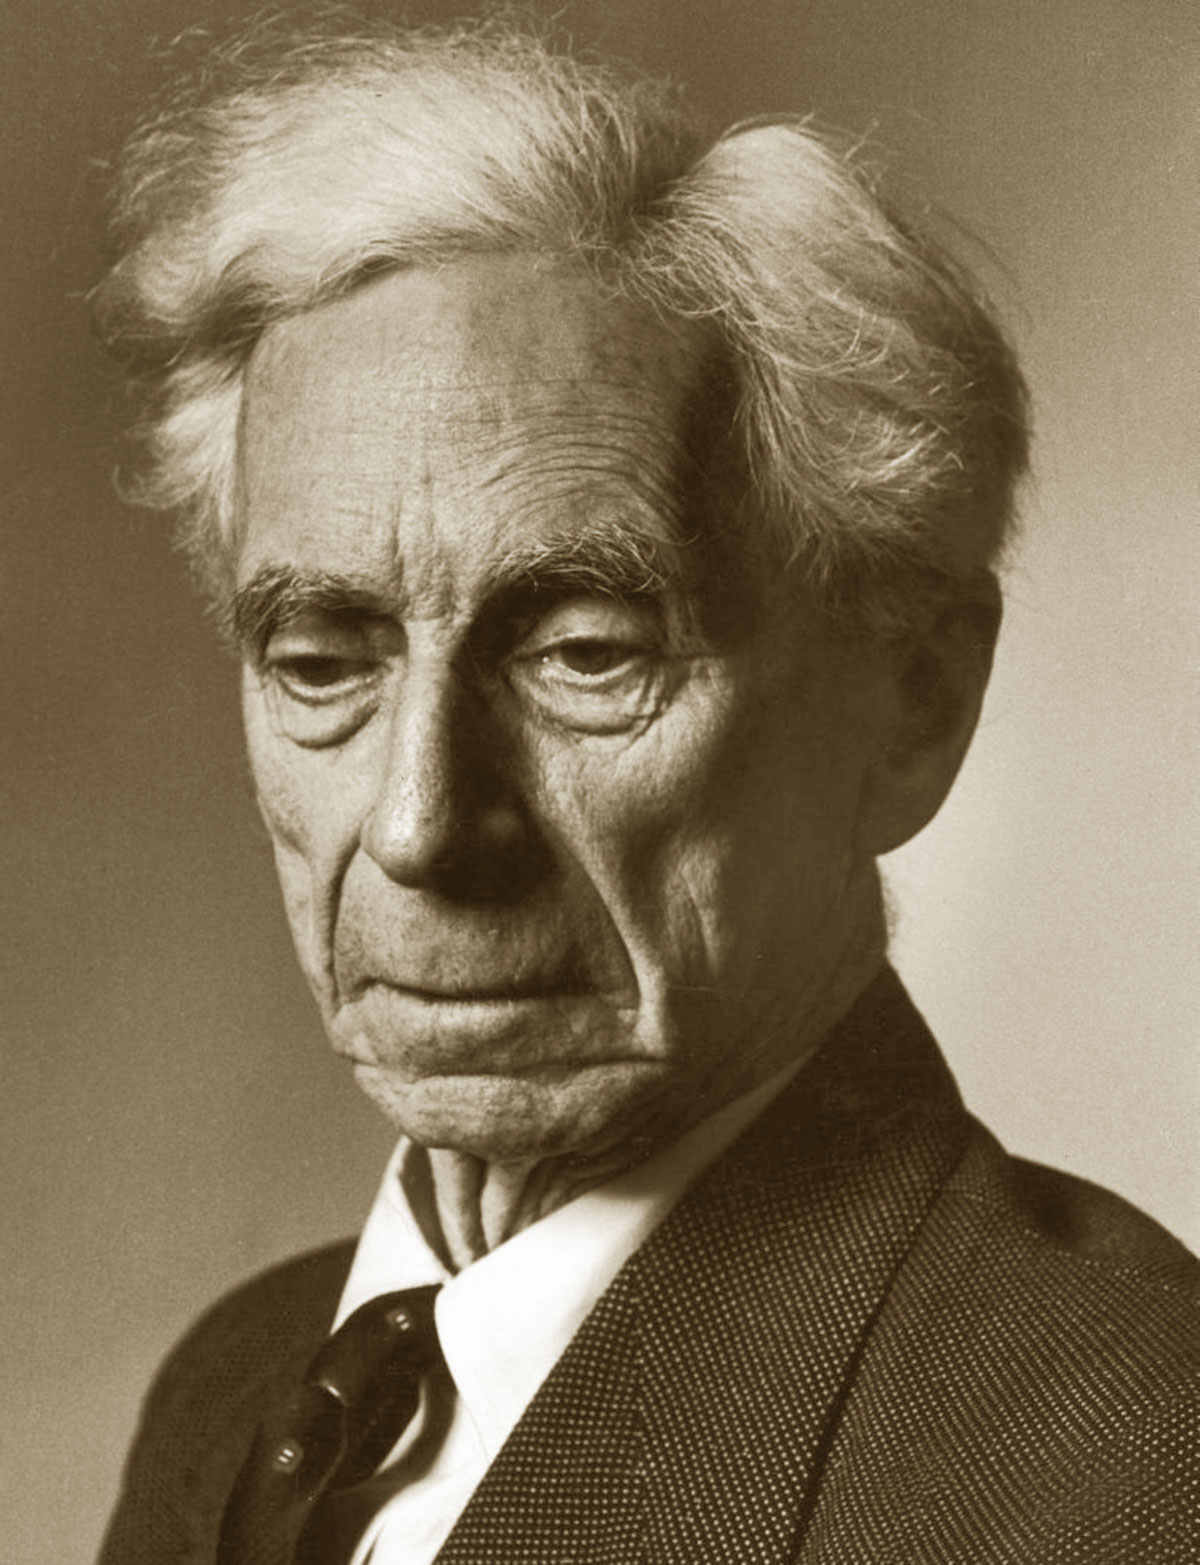
\includegraphics[scale=0.125]{russell}
		\end{center}
\end{frame}

\begin{frame}
		\frametitle{Opérations}
		\begin{center}
				\[
				\begin{prooftree}
						\hypo{A}
						\hypo{B}
						\infer2{C}
				\end{prooftree}
				\]
				\newline
				\[
				A \vdash B
				\]
		\end{center}
\end{frame}

\begin{frame}
\frametitle{Hindley-Milner}
		\[
		\begin{prooftree}
				\hypo{x:\sigma\in\Gamma}
				\infer1[var]{\Gamma \vdash x:\sigma}
		\end{prooftree}
		\]
		\newline
		\[
		\begin{prooftree}
				\hypo{\Gamma, x:\tau \vdash e:\tau'}
				\infer1[abs]{\Gamma \vdash \lambda x.e:\tau \to \tau'}
		\end{prooftree}
		\]
		\newline
		\[
		\begin{prooftree}
				\hypo{\Gamma \vdash f:\tau \to \tau'}
				\hypo{\Gamma \vdash e : \tau}
				\infer2[app]{\Gamma \vdash f\ e : \tau'}
		\end{prooftree}
		\]
\end{frame}

\begin{frame}
		\frametitle{Hindley-Milner}
		\begin{enumerate}
				\item Assignation de variables de types aux expressions
				\item Génération de contraintes
				\item Substitutions
				\item Unification
				\item Instantiation, généralisation
		\end{enumerate}
\end{frame}

\section{Ma démonstration}
\begin{frame}
		\frametitle{Ma démonstration}
\end{frame}

\section{Et après ?}
\begin{frame}
		\frametitle{Et après ?}
		\begin{itemize}
				\item<1-> Est-ce que il y a un réel impact sur la complexité temporelle ?
				\item<2->Pour quelles grammaires est-ce possible ?
				\item<3->Formalisation de cet outil ?
		\end{itemize}
\end{frame}

\end{document}
